% =====================================================================
%  Laboratorio de Metodos Cuantitativos Aplicados a la Gestion - FCE UBA
%  Clase 19 - Simulacion de datos y muestreo
%  Juan Ignacio da Torre - 2do cuatrimestre 2026
%
%  REGLAS DE ESTA PRESENTACION:
%   - Paleta BORDO (la clase la firma Juan solo)
%   - SIN CODIGO: la teoria va aca, el codigo va en el notebook de Colab
%   - La PPT y el notebook se recorren EN PARALELO
%     (notebooks/19_Simulacion_de_datos_y_muestreo.ipynb)
%   - Todos los numeros salen del notebook (semilla fija)
% =====================================================================
\documentclass[aspectratio=169,10pt]{beamer}

\usetheme{CambridgeUS}
\usecolortheme{seahorse}

\definecolor{bordoBase}{HTML}{8B1A1A}
\definecolor{bordoOscuro}{HTML}{5C0A0A}

\setbeamercolor{structure}{fg=bordoBase}
\setbeamercolor{palette primary}{bg=bordoBase!15,fg=black}
\setbeamercolor{palette secondary}{bg=bordoBase!20,fg=black}
\setbeamercolor{palette tertiary}{bg=bordoBase!25,fg=black}
\setbeamercolor{title}{fg=white,bg=bordoOscuro}
\setbeamercolor{author}{fg=black}
\setbeamercolor{institute}{fg=black}
\setbeamercolor{date}{fg=black}
\setbeamercolor{frametitle}{bg=bordoBase!8,fg=bordoOscuro}
\setbeamerfont{frametitle}{series=\bfseries,size=\large}
\setbeamercolor{block title}{bg=bordoBase!15,fg=bordoOscuro}
\setbeamercolor{block body}{bg=bordoBase!5,fg=black}
\setbeamercolor{block title alerted}{bg=bordoBase,fg=white}
\setbeamercolor{block body alerted}{bg=bordoBase!5,fg=black}
\setbeamercolor{block title example}{bg=bordoOscuro,fg=white}
\setbeamercolor{block body example}{bg=bordoBase!5,fg=black}
\setbeamercolor{itemize item}{fg=bordoBase}
\setbeamercolor{itemize subitem}{fg=bordoBase}

\usepackage[utf8]{inputenc}
\usepackage[T1]{fontenc}
\usepackage{lmodern}
\usepackage[spanish,es-tabla,es-nodecimaldot]{babel}
\usepackage{graphicx}
\usepackage{amsmath}
\usepackage{amssymb}
\usepackage{booktabs}
\usepackage{array}
\graphicspath{{imagenes/}}

\title{Simulación de Datos y Muestreo}
\subtitle{Cuánto podemos confiar en una muestra, y cómo simular para averiguarlo}
\author{Juan Ignacio da Torre}
\institute{
    Laboratorio de Métodos Cuantitativos Aplicados a la Gestión \\
    Universidad de Buenos Aires
}
\date{Segundo cuatrimestre 2026}

\setbeamertemplate{footline}[frame number]

\begin{document}

\begin{frame}
\titlepage
\vspace{-0.5cm}
\begin{center}
\textbf{Objetivo:} entender cuánto se equivoca una muestra y qué hacer para que se equivoque poco
\end{center}
\end{frame}

\begin{frame}{Cómo vamos a trabajar}
\begin{block}{Esta presentación va acompañada de un notebook}
Las dos cosas se recorren \textbf{en paralelo}: acá el concepto y la cuenta a mano, y en el notebook lo hacemos correr.
\end{block}
\vspace{0.3cm}
\begin{columns}[T]
\column{0.47\textwidth}
\textbf{En la presentación}
\begin{itemize}
  \item La idea de cada concepto
  \item Las fórmulas, paso a paso
  \item Los resultados que vamos a ver
\end{itemize}
\column{0.47\textwidth}
\textbf{En el notebook}
\begin{itemize}
  \item Una población de 100.000 clientes
  \item Miles de muestras simuladas
  \item Ejercicios con solución
\end{itemize}
\end{columns}
\vspace{0.3cm}
\begin{center}
\small\texttt{notebooks/19\_Simulacion\_de\_datos\_y\_muestreo.ipynb}
\end{center}
\end{frame}

\begin{frame}{De dónde venimos y a dónde vamos}
\begin{columns}[T]
\column{0.45\textwidth}
\begin{block}{Clase 06: cómo muestrear}
Aleatorio simple, porcentual, por filtro, estratificado y por conglomerados, con \texttt{.sample()} de pandas.
\end{block}
\column{0.52\textwidth}
\begin{block}{Hoy: cuánto confiar}
\begin{itemize}
  \item ¿Cuánto se equivoca una muestra?
  \item ¿Qué tamaño necesito?
  \item ¿Cómo elijo para equivocarme menos?
  \item ¿Qué pasa si elijo mal?
\end{itemize}
\end{block}
\end{columns}
\vspace{0.3cm}
\begin{alertblock}{Para responder: simular}
En la vida real no conocemos la verdad. Si \textbf{fabricamos} la población, sí la conocemos, y podemos ver cuánto se equivoca cada muestra.
\end{alertblock}
\end{frame}

% =====================================================================
\section{Muestra y población}
% =====================================================================

\begin{frame}{Población, muestra, parámetro y estadístico}
\begin{columns}[c]
\column{0.40\textwidth}
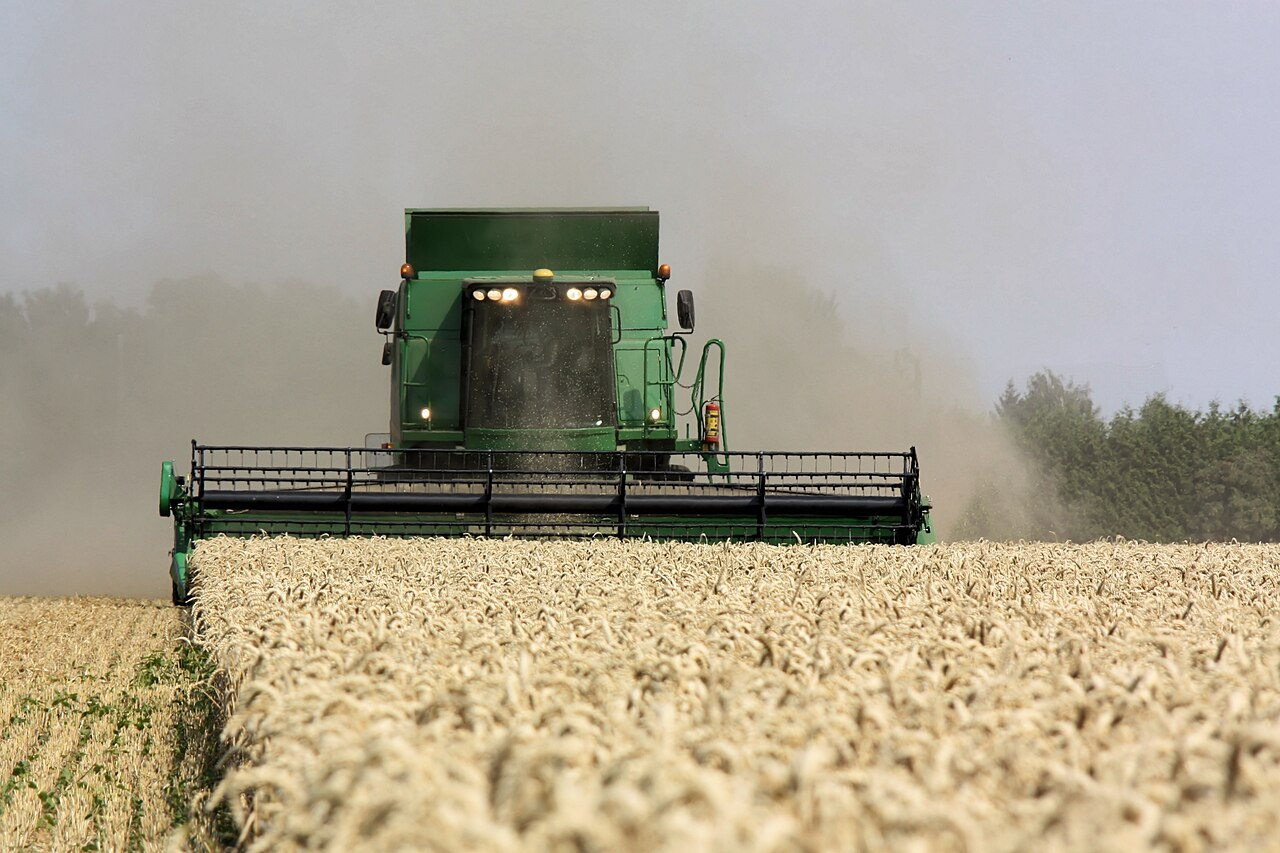
\includegraphics[width=\linewidth]{cosecha_trigo.jpg}
\column{0.56\textwidth}
\begin{tabular}{@{}ll@{}}
\toprule
\textbf{Concepto} & \textbf{Ejemplo} \\
\midrule
Población & los 100.000 clientes \\
Muestra & 100 clientes elegidos \\
Parámetro & gasto promedio verdadero \\
Estadístico & gasto promedio de la muestra \\
\bottomrule
\end{tabular}

\vspace{0.3cm}
\textbf{Error muestral} $=$ estadístico $-$ parámetro.

\small No es una equivocación: es el desvío inevitable por mirar solo una parte.
\end{columns}
\end{frame}

\begin{frame}{Nuestro mundo simulado: la base de clientes}
\begin{center}
\small
\begin{tabular}{@{}lll@{}}
\toprule
\textbf{Variable} & \textbf{Cómo se genera} & \textbf{Valor verdadero} \\
\midrule
Segmento & 60\% Básico · 30\% Medio · 10\% Premium & --- \\
Canal & 35\% Online · 65\% Sucursal & 35,3\% Online \\
Gasto mensual & lognormal: cola larga hacia arriba & \textbf{promedio \$94.566} \\
 & & mediana \$69.984 \\
 & & desvío $\sigma =$ \$74.343 \\
\bottomrule
\end{tabular}
\end{center}
\vspace{0.2cm}
\begin{alertblock}{La semilla}
Los números ``al azar'' de la computadora salen de una fórmula: con la misma \textbf{semilla} salen siempre los mismos. Por eso fijamos una semilla: así el resultado se puede repetir y defender.
\end{alertblock}
\end{frame}

% =====================================================================
\section{Error muestral}
% =====================================================================

\begin{frame}{Una muestra, un error; otra muestra, otro error}
Cinco muestras de 100 clientes, sacadas de la misma población (verdad: \$94.566):

\begin{center}
\begin{tabular}{lcc}
\toprule
\textbf{Muestra} & \textbf{Promedio} & \textbf{Error} \\
\midrule
1 & \$91.874  & $-2.691$ \\
2 & \$111.307 & $+16.741$ \\
3 & \$103.126 & $+8.560$ \\
4 & \$100.016 & $+5.450$ \\
5 & \$90.002  & $-4.564$ \\
\bottomrule
\end{tabular}
\end{center}
\begin{alertblock}{La pregunta}
Cada muestra da un número distinto. ¿Qué tan distintos? Para saberlo: sacar \textbf{mil} muestras.
\end{alertblock}
\end{frame}

\begin{frame}{Mil muestras: la distribución muestral}
Repetimos 1.000 veces con $n = 10$, $n = 100$ y $n = 1.000$, y guardamos cada promedio:

\begin{columns}[T]
\column{0.32\textwidth}
\begin{block}{1. Sin sesgo}
Los promedios se agrupan alrededor del valor verdadero. No se equivocan para ningún lado.
\end{block}
\column{0.32\textwidth}
\begin{block}{2. Más $n$, menos dispersión}
Con $n=10$ los promedios van de un extremo al otro; con $n=1.000$ están pegados a la verdad.
\end{block}
\column{0.32\textwidth}
\begin{block}{3. Forma de campana}
Aunque el gasto tiene cola larga, los \emph{promedios} forman una campana: \textbf{teorema central del límite}.
\end{block}
\end{columns}
\end{frame}

\begin{frame}{El error estándar y la regla de la raíz}
\begin{block}{Error estándar de la media}
\[
EE = \frac{\sigma}{\sqrt{n}}
\]
\end{block}

\begin{columns}[T]
\column{0.54\textwidth}
\textbf{A mano, con $\sigma = 74.343$:}
\[
\begin{aligned}
n = 10:   &\quad \frac{74.343}{\sqrt{10}}   = 23.509 \\[2pt]
n = 100:  &\quad \frac{74.343}{\sqrt{100}}  = 7.434 \\[2pt]
n = 1.000:&\quad \frac{74.343}{\sqrt{1.000}} = 2.351
\end{aligned}
\]
\column{0.42\textwidth}
\begin{center}
\small
\begin{tabular}{rcc}
\toprule
$n$ & \textbf{Simulado} & \textbf{Teórico} \\
\midrule
10 & 22.627 & 23.509 \\
100 & 7.306 & 7.434 \\
1.000 & 2.362 & 2.351 \\
\bottomrule
\end{tabular}
\end{center}
\end{columns}
\vspace{0.2cm}
\begin{alertblock}{Para dividir el error por 2, hay que cuadruplicar la muestra}
$n$ está dentro de una raíz: $\sqrt{4n} = 2\sqrt{n}$.
\end{alertblock}
\end{frame}

% =====================================================================
\section{Tamaño de muestra}
% =====================================================================

\begin{frame}{¿Qué tamaño de muestra necesito?}
Con confianza del 95\%, la estimación cae a menos de $1{,}96$ errores estándar de la verdad:
\[
\text{margen de error} = 1{,}96 \cdot \frac{\sigma}{\sqrt{n}}
\]
\begin{center}
\small
\begin{tabular}{rccc}
\toprule
$n$ & \textbf{Error estándar} & \textbf{Margen (95\%)} & \textbf{Margen en \% del promedio} \\
\midrule
25 & 14.869 & 29.142 & 30,8\% \\
100 & 7.434 & 14.571 & 15,4\% \\
400 & 3.717 & 7.286 & 7,7\% \\
1.600 & 1.859 & 3.643 & 3,9\% \\
6.400 & 929 & 1.821 & 1,9\% \\
\bottomrule
\end{tabular}
\end{center}
Cada fila cuadruplica a la anterior y el margen se divide a la mitad.
\end{frame}

\begin{frame}{Para una proporción: el caso de las encuestas}
\[
\text{margen} = 1{,}96\sqrt{\frac{p(1-p)}{n}}
\qquad\Longrightarrow\qquad
n = \frac{1{,}96^2\, p\,(1-p)}{\text{margen}^2}
\]
\begin{columns}[T]
\column{0.55\textwidth}
\textbf{A mano:} sin idea de $p$ se usa el peor caso, $p = 0{,}5$. Margen $\pm 3\%$:
\[
n = \frac{3{,}8416 \times 0{,}25}{0{,}03^2} = \frac{0{,}9604}{0{,}0009} \approx 1.068
\]
\column{0.40\textwidth}
\begin{center}
\small
\begin{tabular}{lr}
\toprule
\textbf{Caso} & \textbf{n} \\
\midrule
$p=0{,}5$, $\pm 3\%$ & 1.068 \\
$p=0{,}35$, $\pm 2\%$ & 2.185 \\
$p=0{,}5$, $\pm 1\%$ & 9.604 \\
\bottomrule
\end{tabular}
\end{center}
\end{columns}
\vspace{0.2cm}
\begin{alertblock}{Lo que sorprende}
El tamaño de la población casi no importa: para el mismo margen, una ciudad de 100.000 y un país de 40 millones necesitan prácticamente la misma muestra. Importa la \textbf{precisión} que querés.
\end{alertblock}
\end{frame}

% =====================================================================
\section{Cómo se muestrea}
% =====================================================================

\begin{frame}{Cinco maneras de elegir a quién preguntar}
\small
\begin{center}
\begin{tabular}{@{}lp{6.2cm}@{}}
\toprule
\textbf{Método} & \textbf{Cómo se elige} \\
\midrule
Aleatorio simple & Todos tienen la misma chance: sorteo de toda la lista \\
Estratificado por segmento & Grupos Básico, Medio y Premium; se sortea dentro de cada uno, en proporción a su peso (120, 60 y 20 de 200) \\
Estratificado por ciudad & Lo mismo, con una cuota por ciudad \\
Sistemático & Uno cada $k$ de la lista, con arranque al azar \\
Por conveniencia & A quien es fácil de alcanzar: acá, solo los clientes Online \\
\bottomrule
\end{tabular}
\end{center}
\vspace{0.1cm}
\small Comparamos $n=200$, repetido 2.000 veces con cada método. Verdad: \$94.566.
\end{frame}

\begin{frame}{Quién se equivoca más, y para dónde}
\begin{center}
\begin{tabular}{lccc}
\toprule
\textbf{Método} & \textbf{Promedio de las estimaciones} & \textbf{Sesgo} & \textbf{Desvío entre muestras} \\
\midrule
Aleatorio simple & 94.723 & $+158$ & 5.199 \\
\textbf{Estratificado por segmento} & 94.633 & $+67$ & \textbf{3.043} \\
Estratificado por ciudad & 94.524 & $-42$ & 5.280 \\
Sistemático & 94.479 & $-87$ & 5.247 \\
\textbf{Por conveniencia (Online)} & \textbf{110.515} & \textbf{$+15.949$} & 5.894 \\
\bottomrule
\end{tabular}
\end{center}
\vspace{0.2cm}
\begin{columns}[T]
\column{0.48\textwidth}
\begin{block}{Estratificar por segmento}
Baja el error un \textbf{41\%}: los segmentos son muy distintos entre sí, y asegurar que cada uno esté en su proporción elimina la variación de ``cuántos premium me tocaron''.
\end{block}
\column{0.48\textwidth}
\begin{block}{Estratificar por ciudad}
\textbf{No mejora nada}: las ciudades gastan lo mismo. Se estratifica por una variable \emph{relacionada} con lo que se mide.
\end{block}
\end{columns}
\end{frame}

\begin{frame}{El sesgo no se arregla con más datos}
\begin{columns}[c]
\column{0.50\textwidth}
Muestra por conveniencia: solo clientes Online.
\begin{center}
\begin{tabular}{rc}
\toprule
\textbf{n} & \textbf{Error vs. la verdad} \\
\midrule
200 & $+12.919$ \\
1.000 & $+18.869$ \\
5.000 & $+15.509$ \\
20.000 & $+15.927$ \\
\bottomrule
\end{tabular}
\end{center}
\column{0.46\textwidth}
\begin{alertblock}{La lección}
Más $n$ achica el error \textbf{aleatorio}, pero no toca el error \textbf{sistemático}.

Una muestra grande y mal elegida da una respuesta equivocada \textbf{con mucha confianza}.
\end{alertblock}
\end{columns}
\vspace{0.2cm}
\small Es el error clásico de las encuestas por redes, los comentarios de una app o ``los clientes que se quejan''.
\end{frame}

% =====================================================================
\section{Monte Carlo}
% =====================================================================

\begin{frame}{Simulación de Monte Carlo}
\begin{block}{La idea, en cuatro pasos}
\begin{enumerate}
  \item Definir un modelo con variables \textbf{inciertas}.
  \item \textbf{Sortear} valores para esas variables, miles de veces.
  \item Calcular el resultado en cada sorteo.
  \item Mirar la \textbf{distribución} de resultados, no un solo número.
\end{enumerate}
\end{block}
\vspace{0.2cm}
\textbf{Calentamiento:} estimar $\pi$ tirando 100.000 puntos al azar en un cuadrado de lado 1. El cuarto de círculo ocupa $\pi/4$ del cuadrado, así que
\[
\frac{\text{puntos adentro}}{\text{total}} \approx \frac{\pi}{4} \quad\Rightarrow\quad \pi \approx 4 \times 0{,}7855 = 3{,}1421
\]
\end{frame}

\begin{frame}{El horno de la panadería, con incertidumbre}
\begin{columns}[c]
\column{0.36\textwidth}
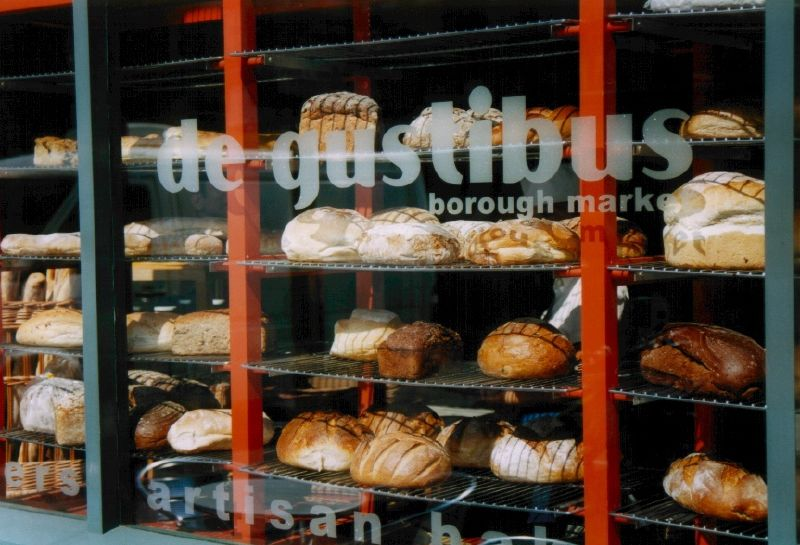
\includegraphics[width=\linewidth]{panaderia.jpg}
\column{0.60\textwidth}
Clase 14: inversión de \$10 millones, flujos $3 / 3{,}5 / 4 / 4 / 3$, costo de capital 20\%.
\[
VAN = -10 + \frac{3}{1{,}2} + \frac{3{,}5}{1{,}2^2} + \frac{4}{1{,}2^3} + \frac{4}{1{,}2^4} + \frac{3}{1{,}2^5} = +0{,}38
\]
Conviene, pero \emph{por poco}. Esa cuenta supone que los flujos serán \textbf{exactamente} esos.

Si cada flujo varía un 20\% alrededor de lo esperado, y simulamos 20.000 futuros:
\end{columns}
\end{frame}

\begin{frame}{¿Qué dice la simulación?}
\begin{columns}[T]
\column{0.50\textwidth}
\begin{center}
\begin{tabular}{lr}
\toprule
VAN promedio simulado & +0,38 M \\
Desvío del VAN & 0,96 M \\
Rango central 90\% & $-1{,}20$ a $+1{,}95$ M \\
\textbf{Probabilidad de VAN $<$ 0} & \textbf{34,5\%} \\
\bottomrule
\end{tabular}
\end{center}
\column{0.46\textwidth}
\begin{alertblock}{Moraleja}
Un VAN de $+0{,}38$ parecía un buen proyecto. Con incertidumbre, hay \textbf{una chance de cada tres} de perder plata.

Monte Carlo no reemplaza al VAN: lo \textbf{completa} con la pregunta \emph{``¿qué tan seguro es?''}
\end{alertblock}
\end{columns}
\vspace{0.2cm}
\small Es lo que hicimos con Stargate Argentina: en vez de ``2,8\% de la demanda'', simulamos 10.000 escenarios y dijimos ``entre 2,3\% y 3,3\%''.
\end{frame}

\begin{frame}{Más incertidumbre, más riesgo}
\begin{center}
\begin{tabular}{ccc}
\toprule
\textbf{Desvío de los flujos} & \textbf{VAN promedio} & \textbf{Probabilidad de perder} \\
\midrule
0\% & +0,38 & 0\% \\
10\% & 0,38 & 20,9\% \\
20\% & 0,39 & 34,2\% \\
30\% & 0,38 & 39,6\% \\
40\% & 0,37 & 42,1\% \\
\bottomrule
\end{tabular}
\end{center}
El VAN \textbf{promedio} casi no cambia, pero la probabilidad de perder crece con la incertidumbre.
\end{frame}

% =====================================================================
\section{Bootstrap y cierre}
% =====================================================================

\begin{frame}{Bootstrap: remuestrear una sola muestra}
En la vida real tenemos \textbf{una} muestra, no la población. El truco: sacar \emph{de la muestra} nuevas muestras \textbf{con reposición}, del mismo tamaño, y ver cuánto varía el promedio.

\vspace{0.2cm}
\begin{center}
\small
\begin{tabular}{lcc}
\toprule
 & \textbf{Desde} & \textbf{Hasta} \\
\midrule
Promedio de la muestra (n = 200) & \multicolumn{2}{c}{\$105.430} \\
Intervalo 95\% por bootstrap & \$93.167 & \$119.559 \\
Intervalo 95\% por fórmula & \$92.380 & \$118.481 \\
\midrule
Promedio verdadero (no lo conocíamos) & \multicolumn{2}{c}{\textbf{\$94.566}} \\
\bottomrule
\end{tabular}
\end{center}
Sin ninguna fórmula, el bootstrap da un intervalo casi igual, y que \textbf{contiene} a la verdad. Sirve incluso donde no hay fórmula (una mediana, un cociente).
\end{frame}

\begin{frame}{Para llevarse}
\begin{enumerate}
  \item \textbf{Fijá la semilla}: sin ella no se puede repetir ni defender un resultado.
  \item Una muestra aleatoria se equivoca \textbf{poco} (y menos cuanto más grande) y \textbf{sin sesgo}.
  \item Para \textbf{dividir el error por 2}, cuadruplicá la muestra.
  \item \textbf{Estratificá} por una variable relacionada con lo que medís; si no, no mejora nada.
  \item El \textbf{sesgo no se arregla con más datos}: desconfiá de ``la gente que respondió''.
  \item \textbf{Monte Carlo} mide el riesgo de una decisión: simular miles de futuros y mirar la distribución.
\end{enumerate}
\end{frame}

\begin{frame}{En el trabajo práctico}
\small
\begin{center}
\begin{tabular}{@{}p{5.2cm}p{7.2cm}@{}}
\toprule
\textbf{Si en tu TP...} & \textbf{Hacé esto} \\
\midrule
El dataset es enorme y tarda & Explorá con una muestra aleatoria \textbf{con semilla}, y confirmá al final con todo \\
Hay un grupo chico pero importante & \textbf{Estratificá}, para que no desaparezca \\
Los datos vienen de una encuesta o app & Preguntate \textbf{quién respondió} \\
Querés probar el código antes de los datos & \textbf{Simulá} datos con la misma forma \\
Vas a mostrar un promedio o un \% & Acompañalo con su \textbf{margen de error} \\
\bottomrule
\end{tabular}
\end{center}
\small En la metodología del informe, decí \textbf{cómo se obtuvieron los datos}: quién los generó, cuántos son y si son toda la población o una muestra.
\end{frame}

\begin{frame}{Ejercicios (en el notebook, con solución)}
\begin{enumerate}
  \item \textbf{Dados.} Simulá 100.000 tiradas de dos dados: ¿con qué frecuencia suman 7? Compará con $6/36$.
  \item \textbf{Tamaño de muestra.} ¿Qué $n$ estima la proporción de clientes Online con $\pm 2\%$? Verificalo con 1.000 muestras.
  \item \textbf{Estratificar o no.} Repetí la comparación estratificando por canal. ¿Mejora? ¿Por qué?
  \item \textbf{Monte Carlo.} En el horno, ¿qué probabilidad de perder hay si el costo de capital sube al 25\%?
\end{enumerate}
\end{frame}

\begin{frame}{Preguntas}
\vspace{2cm}
\begin{center}
\Huge ¿Preguntas?
\end{center}
\end{frame}

\begin{frame}{Fuentes}
\small
\begin{itemize}
  \item Moore, D., McCabe, G., \& Craig, B. (2017). \emph{Introduction to the Practice of Statistics} (9th ed.). W. H. Freeman.
  \item Lohr, S. (2021). \emph{Sampling: Design and Analysis} (3rd ed.). CRC Press.
  \item Efron, B., \& Tibshirani, R. (1993). \emph{An Introduction to the Bootstrap}. Chapman \& Hall.
  \item Brealey, R., Myers, S., \& Allen, F. (2020). \emph{Principles of Corporate Finance} (13th ed.). McGraw-Hill. (Simulación de Monte Carlo en la evaluación de proyectos.)
  \item Clases 06 (muestreo), 14 (VAN y métricas) y 21 (métricas estadísticas) de este laboratorio.
\end{itemize}
\end{frame}

\end{document}
